\chapter{Implementation}

\section{Backend Implementation}
The backend of Slotify is robustly built using Node.js and Express.js, providing a highly performant, non-blocking runtime environment ideal for handling numerous concurrent booking requests. This server-side layer acts as the authoritative engine of the platform: it meticulously manages token-based authentication, orchestrates complex appointment processing and slot validation, executes fast geospatial and textual service queries, and strictly enforces all business logic constraints. To ensure that the codebase remains clean, testable, and deeply scalable as the project scope inevitably grows, a structured routing and controller architectural pattern is strictly adhered to. This clearly separates the definition of API endpoints from the actual business logic that executes when those endpoints are called.

\subsection{Project Structure}
The backend project directory is meticulously organized into discrete, modular folders such as controllers (for business logic), models (for database schemas and Mongoose wrappers), middleware (for request interception and validation), routes (for endpoint definitions), and utilities (for shared helper functions like date parsing). This strict logical separation allows the development team to manage core business logic, strict data validation before database insertion, and optimized database access queries much more efficiently. A clean, predictable project structure is absolutely essential in a complex platform that simultaneously supports multiple distinct user roles (admin, staff, customer) and dynamically changing services across different independent tenant businesses.

\begin{figure}[h]
\centering
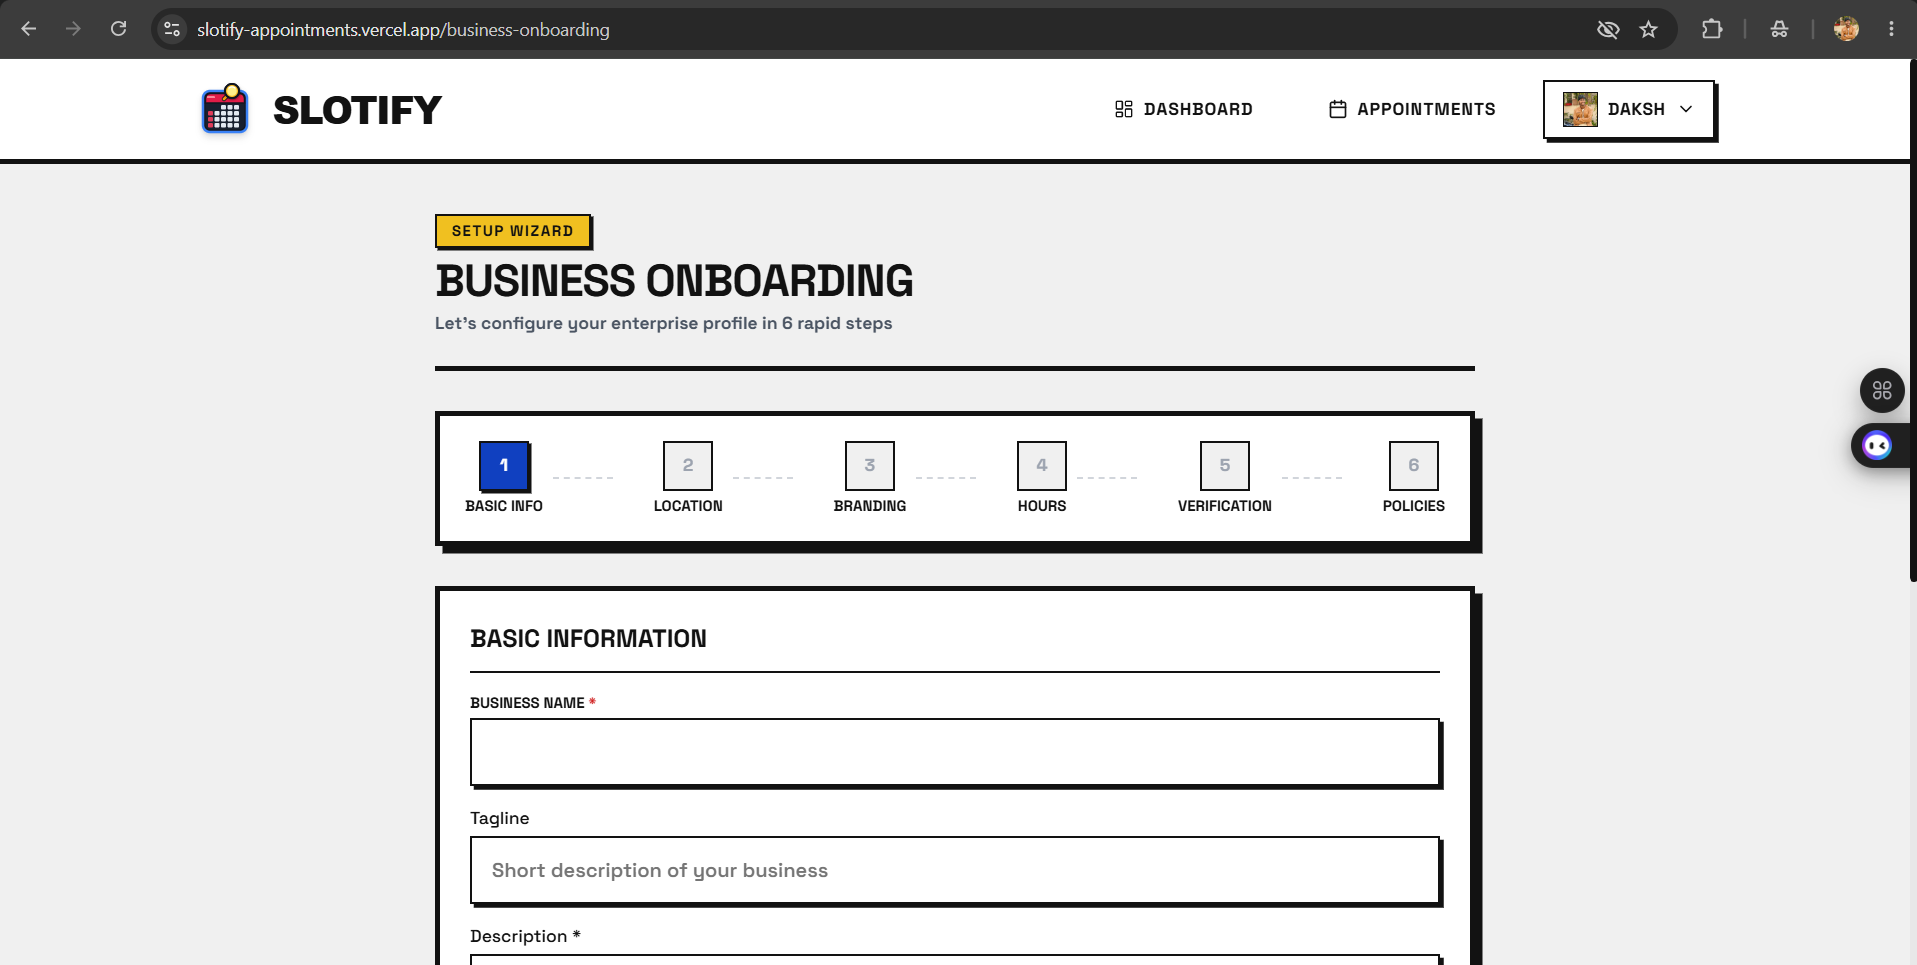
\includegraphics[width=0.8\textwidth]{images/business setup.png}
\caption{Business configuration and setup screen}
\end{figure}

\begin{figure}[h]
\centering
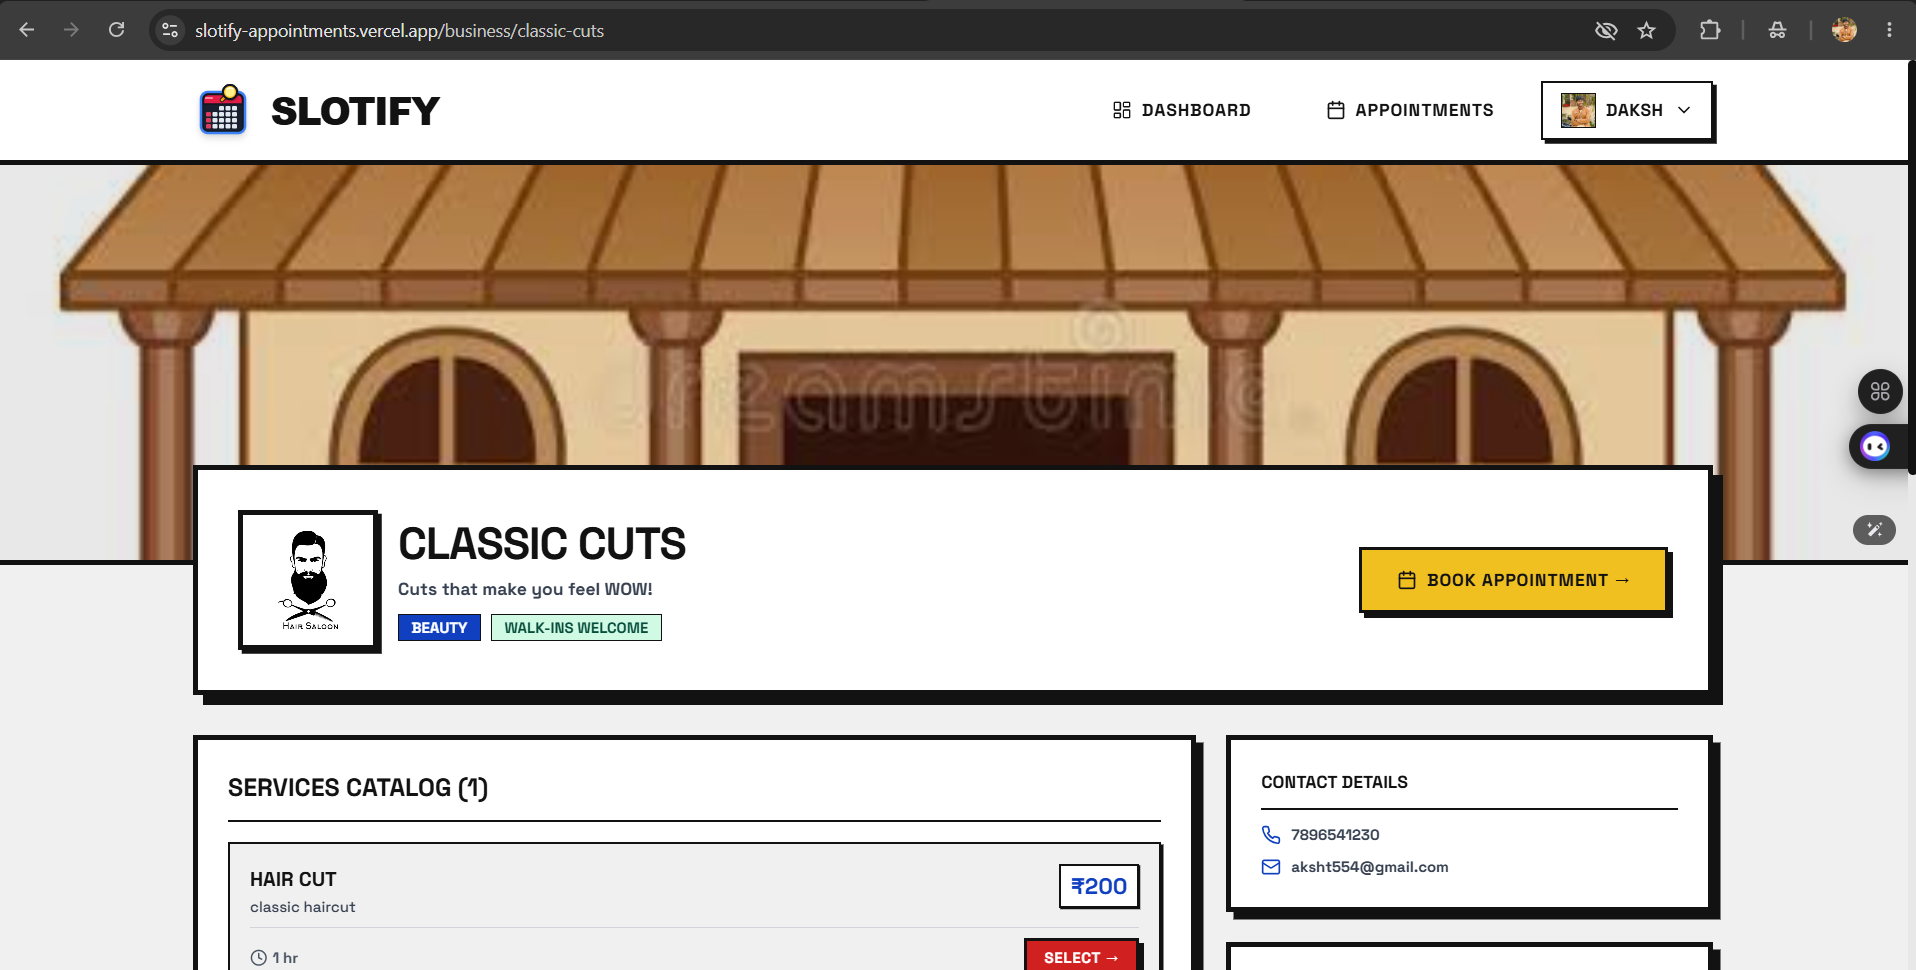
\includegraphics[width=0.8\textwidth]{images/business.png}
\caption{Business profile and service discovery interface}
\end{figure}

\subsection{Slot Availability Logic}
The core slot availability engine is arguably the most complex and critical piece of logic in the backend. When queried, it dynamically cross-references and evaluates a multitude of factors: the overarching business working hours, individual staff shift schedules and breaks, holiday block-outs, and all currently existing confirmed or pending bookings. It uses strict mathematical rules—such as exact service duration, required buffer times between appointments, business cancellation policies, and real-time staff availability—to algorithmically determine and return only mathematically valid appointment windows. This robust, server-side logic strictly prevents race conditions, permanently stops double-booking conflicts, and maintains the absolute operational reliability of the entire booking system.

\subsection{Authentication Middleware}
Custom authentication and authorization middleware systematically verify a user's cryptographic identity (via JWT) before allowing any access to protected API endpoints. This middleware explicitly ensures that users are actively logged in, that their session has not expired, and crucially, that they have the precise role-based authorization required to view or modify the requested business data. For instance, a customer cannot access staff schedules, and one business admin cannot query another business's revenue. This strict gateway is paramount for proactively preventing unauthorized malicious actions and seamlessly enforcing multi-tenant data privacy.

\subsection{Email Notification Service}
The system integrates a dedicated, asynchronous email notification service (utilizing Nodemailer) designed to automatically dispatch rich HTML confirmation messages immediately upon booking, and perfectly timed reminders to customers prior to their appointments. These proactive notifications serve a dual purpose: they dramatically reduce the incidence of costly missed appointments (no-shows) and simultaneously improve the professional communication standard between the small business and the customer. The service is deeply and asynchronously integrated into the booking and state-change flows (such as cancellations or rescheduling) to keep the entire scheduling process transparent and highly reliable without slowing down the immediate API response time for the user.

\section{Frontend Implementation}
The client-facing frontend is entirely built using React, a declarative JavaScript library which provides an exceptionally responsive, fluid, and highly interactive single-page application (SPA) interface for all interacting actors: customers, business admins, and staff members. It is specifically designed to present a completely frictionless, visually clear booking flow, instantly render dynamically available time slots without page reloads, and elegantly manage complex user state across dozens of different views and interactive dashboards.

\subsection{Project Structure}
The frontend codebase is methodically organized into reusable UI components, dedicated page views, dynamic React Router routes, and global context-based state management providers. This highly modular structure vastly improves long-term maintainability, encourages code reuse, and allows the UI to scale elegantly without becoming a tangled mess as new features are integrated into the platform. It also deliberately keeps the distinct functional areas—such as the public landing pages, the secure login portal, the customer booking wizard, and the data-heavy business management dashboards—strictly separated into well-defined, lazy-loaded modules for optimal load performance.

\begin{figure}[h]
\centering
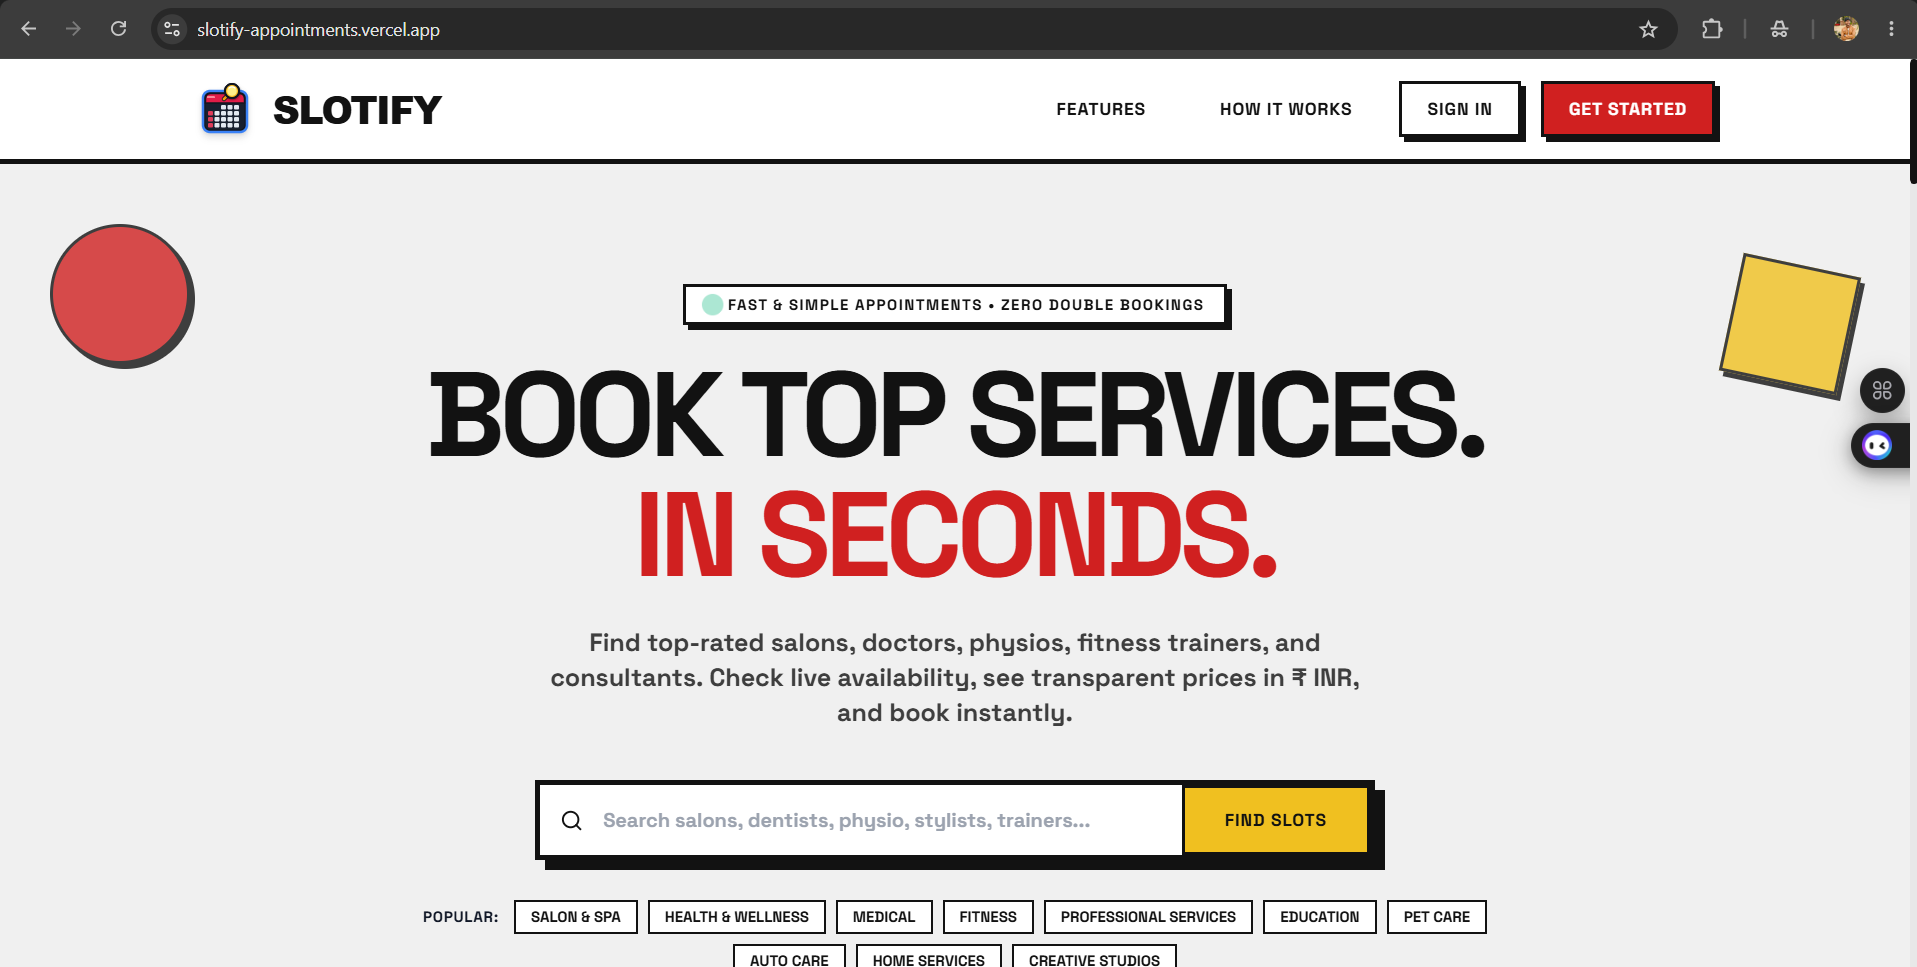
\includegraphics[width=0.8\textwidth]{images/landing page.png}
\caption{Landing page of the Slotify platform}
\end{figure}

\begin{figure}[h]
\centering
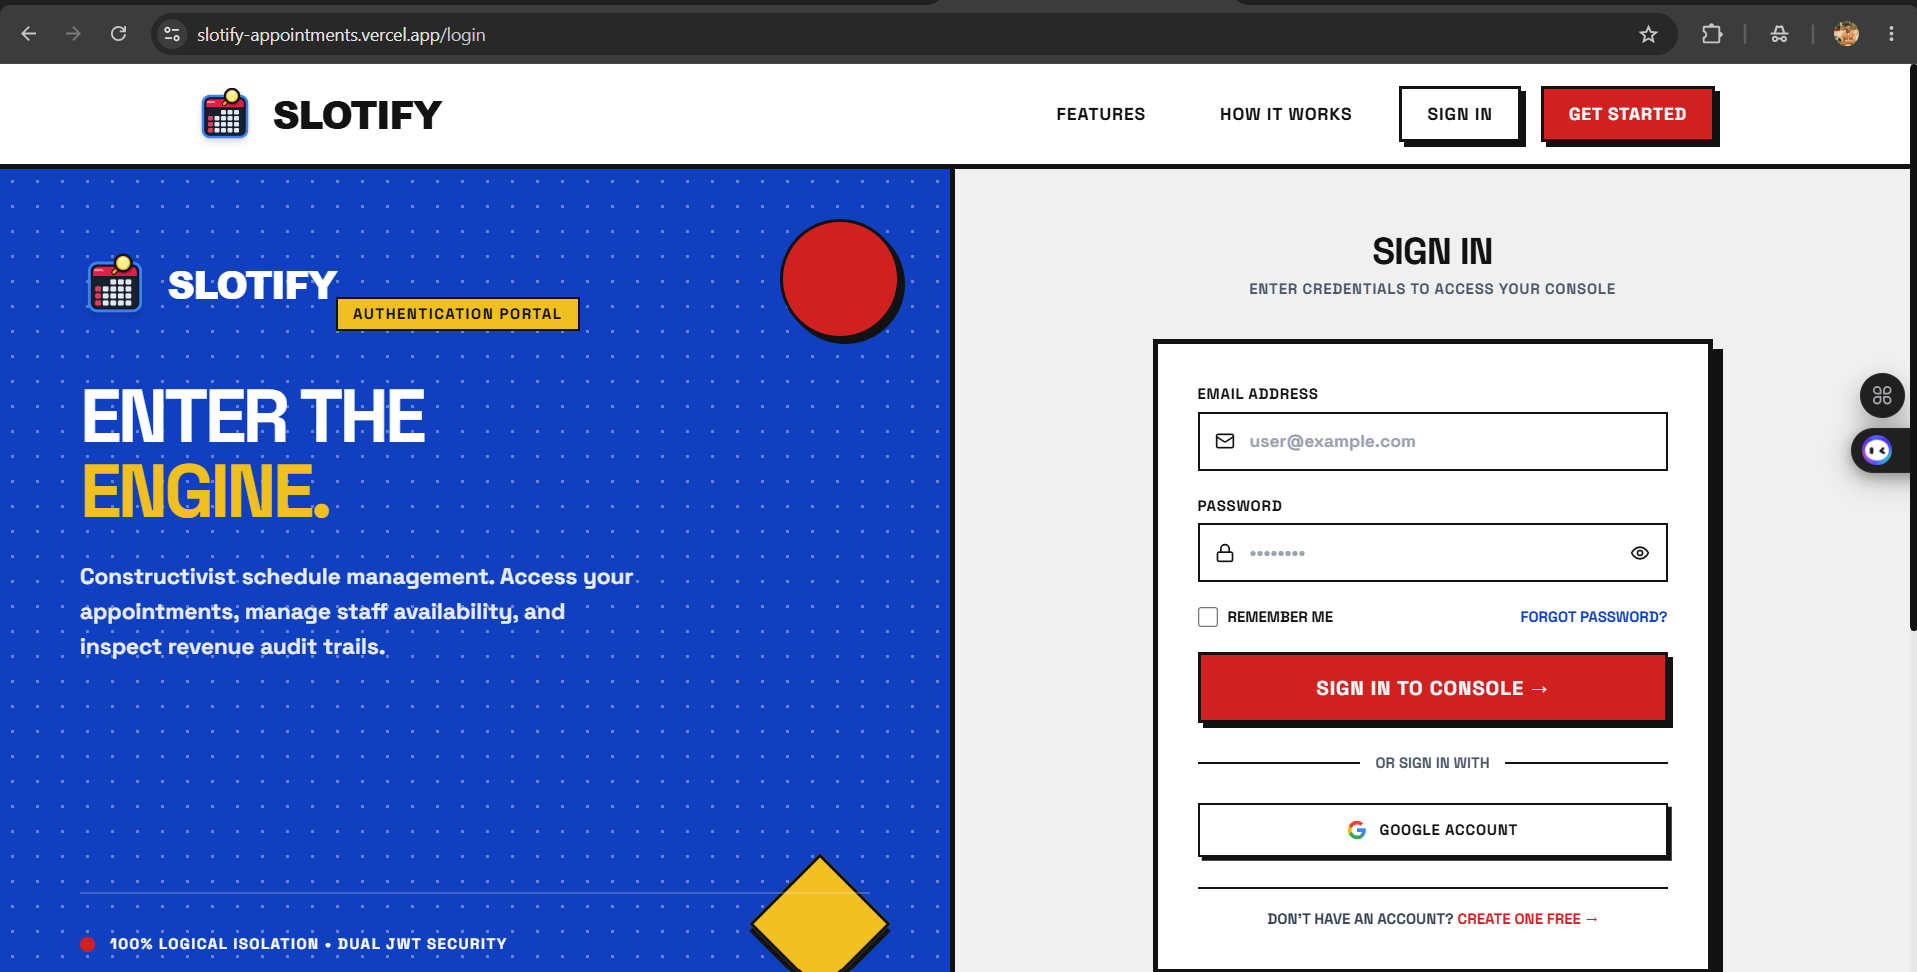
\includegraphics[width=0.8\textwidth]{images/login page.png}
\caption{Login interface for the user authentication flow}
\end{figure}

\subsection{Real-Time Slot Display}
The customer-facing booking interface queries the backend and visually updates the calendar of available time slots dynamically, reacting instantly based on current real-time data and configured business rules. Consequently, customers only ever see mathematically valid, bookable appointment times, which drastically improves the user experience by completely eliminating the frustration and back-and-forth communication typically associated with manual, phone-based scheduling. This seamless, highly accurate real-time slot display is arguably the core operational value proposition of the entire platform, directly bridging the gap between customer convenience and business efficiency.

\begin{figure}[h]
\centering
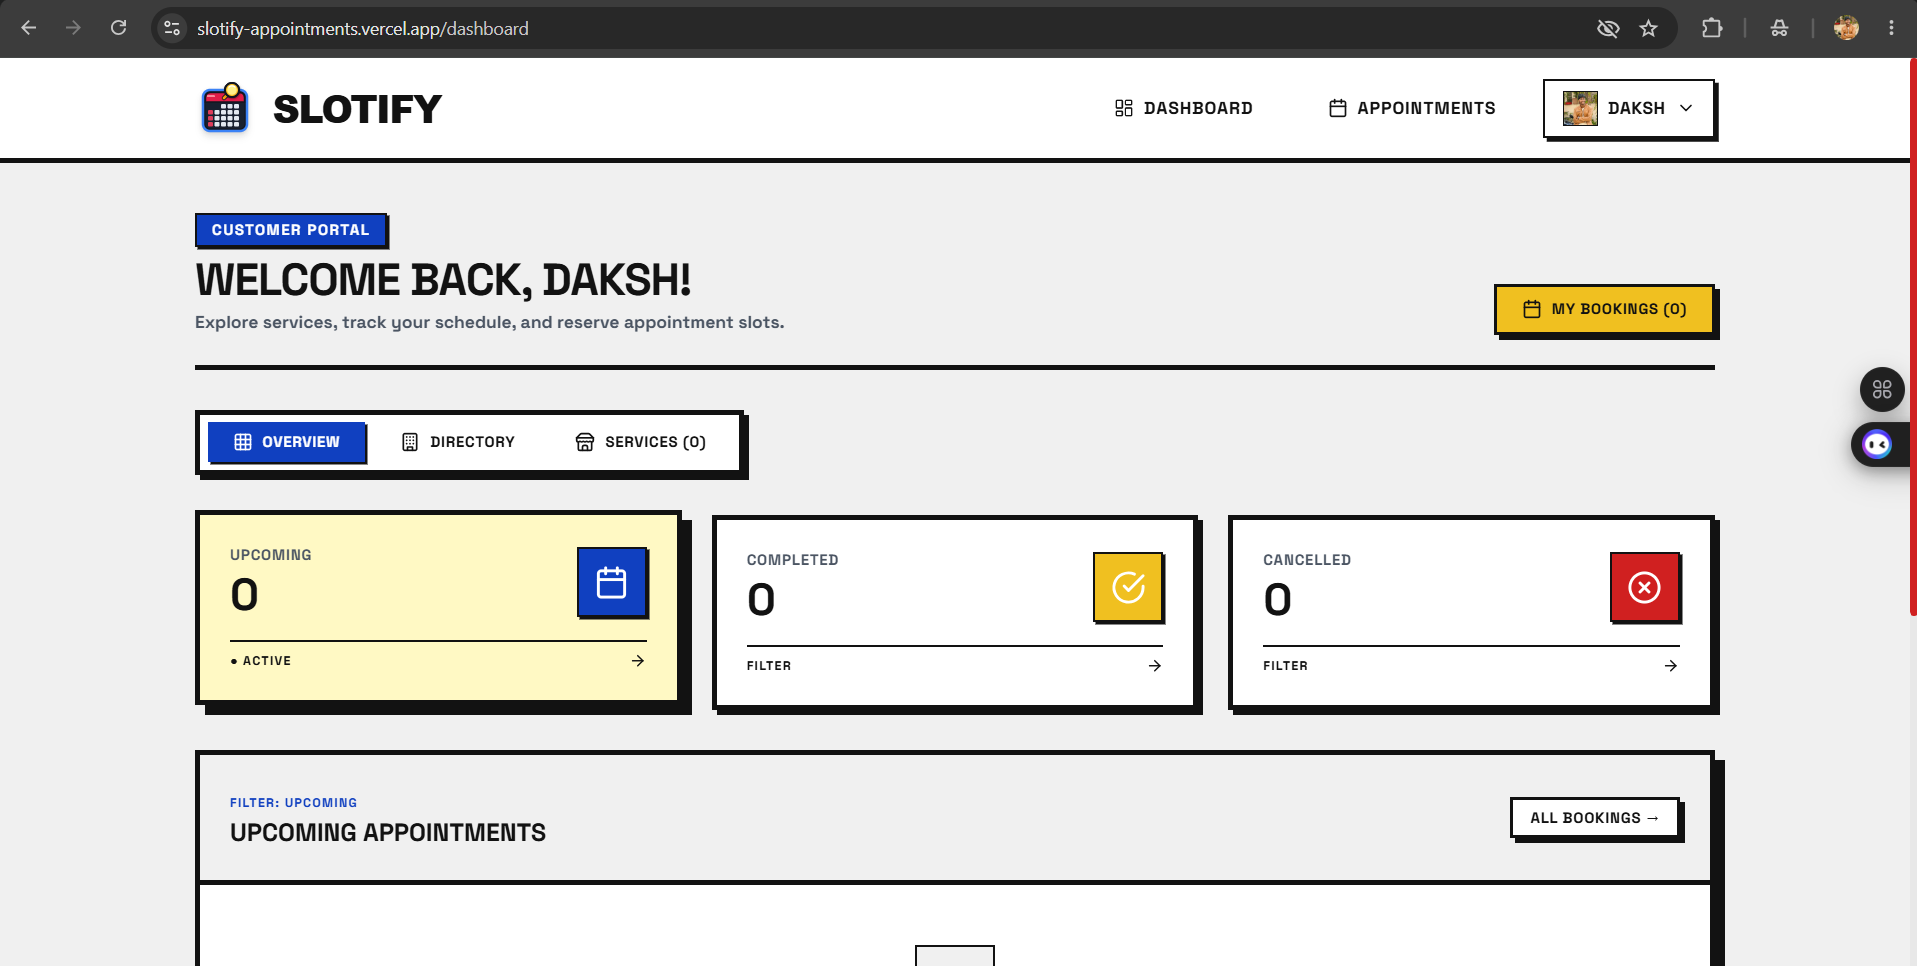
\includegraphics[width=0.85\textwidth]{images/dashboard.png}
\caption{Admin dashboard showing bookings, activities, and business overview}
\end{figure}

\begin{figure}[h]
\centering
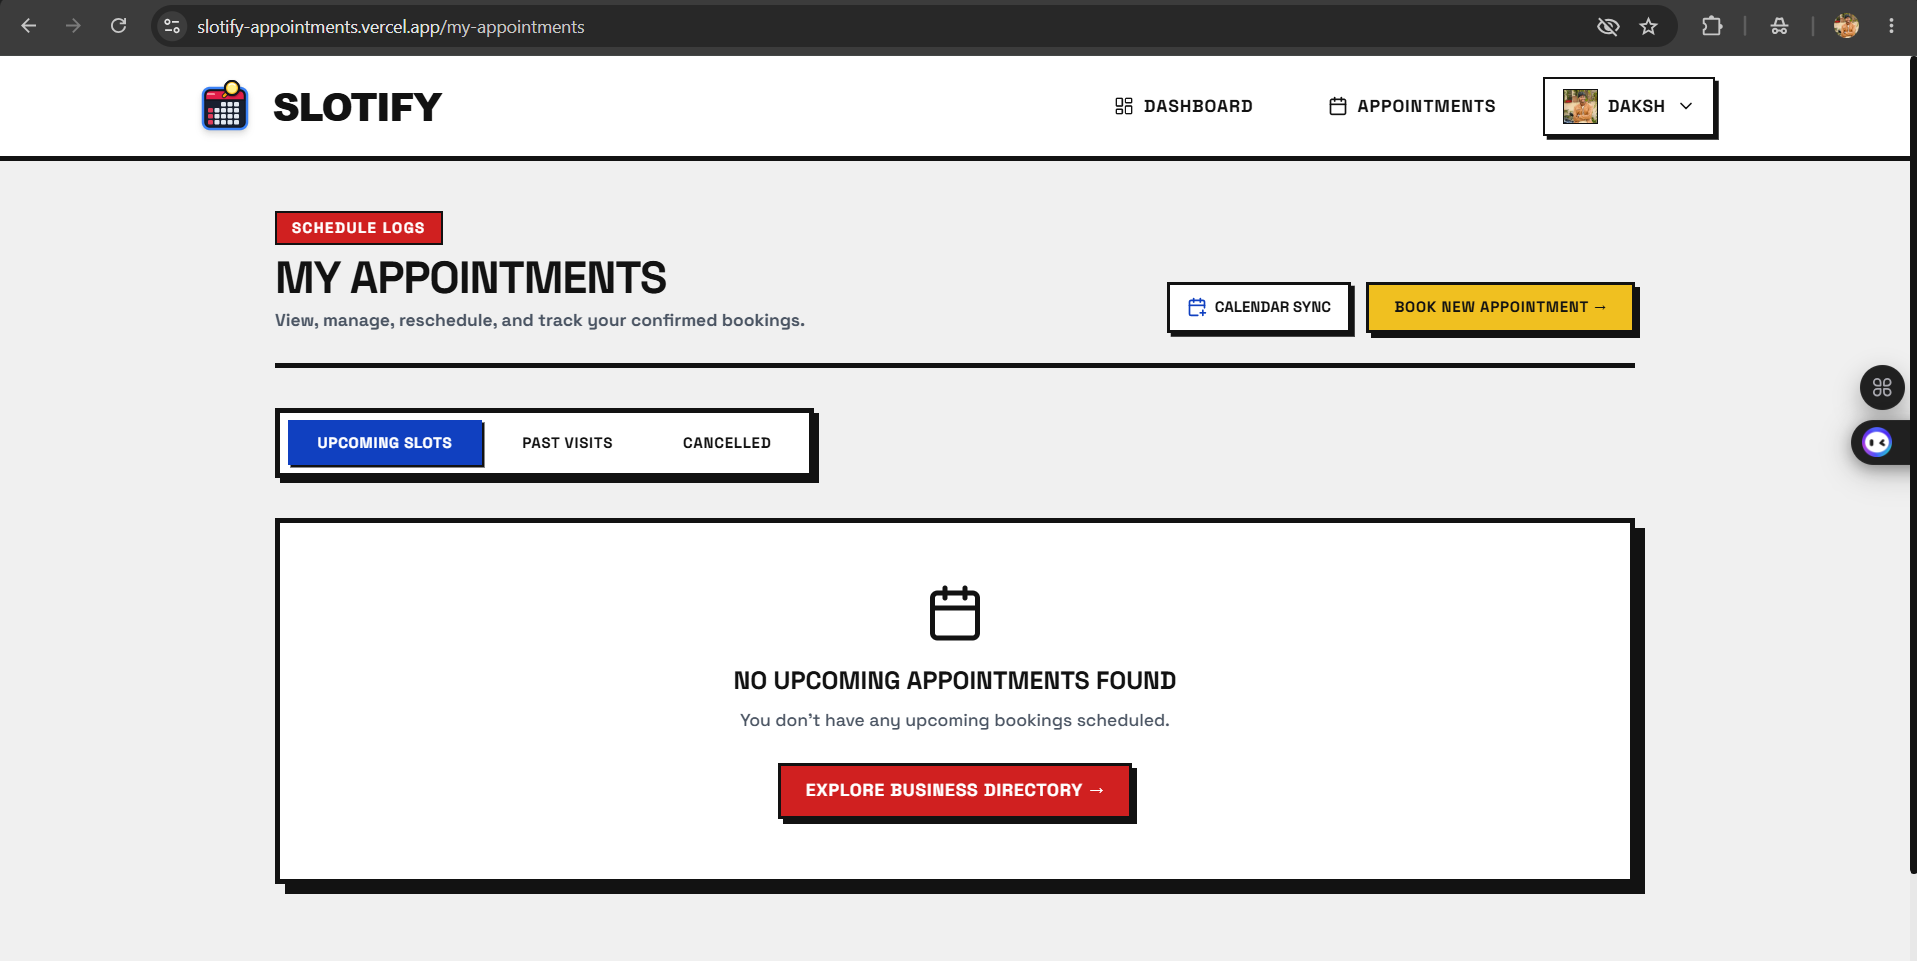
\includegraphics[width=0.85\textwidth]{images/appoinments.png}
\caption{Appointment list and scheduling records}
\end{figure}

\subsection{State Management and Prop Drilling Refactor}
As the React application naturally grew in complexity and feature depth, managing component state became increasingly difficult. The project proactively addressed this technical debt by refactoring the component tree to sharply reduce unnecessary "prop drilling" (passing data through multiple layers of components that do not need it) and instead centralizing critical shared state using React Context APIs where appropriate. This strategic refactoring made the frontend application significantly more maintainable, easier to debug, and vastly improved the consistency and synchronization of critical data—such as the current user's authentication status, selected booking parameters, and real-time dashboard metrics—across the entire component hierarchy.

\section{Implementation Status}
At its current milestone, the application has successfully implemented all the core foundational features required for a fully functional, production-ready booking system. This explicitly includes secure user authentication, geographic and category-based business discovery, dynamic service booking with conflict prevention, automated email reminders, and comprehensive scheduling logic for staff. The project is currently in a highly stable, working state and powerfully demonstrates the commercial viability and technical feasibility of this digital solution tailored specifically for small service-based businesses. Further advanced enhancements—such as integrated Stripe payment processing, AI-driven slot recommendation algorithms for yield management, and dedicated native mobile applications—are meticulously documented and strategically deferred to be added as future phase extensions.

\begin{table}[h]
\centering
\caption{Feature implementation status}
\begin{tabular}{|p{6cm}|p{3cm}|p{3cm}|}
\hline
\textbf{Feature} & \textbf{Status} & \textbf{Phase} \\
\hline
User registration and login & Done & Semester 6 \\
\hline
Real-time slot booking & Done & Semester 6 \\
\hline
Email confirmation and reminder & Done & Semester 6 \\
\hline
Provider dashboard and schedule & Done & Semester 6 \\
\hline
Business analytics & Partial & Semester 6 \\
\hline
Calendar synchronisation & In progress & Semester 6/7 \\
\hline
Payment integration, mobile app, and AI recommendations & Deferred & Semester 7 \\
\hline
\end{tabular}
\end{table}

\begin{figure}[h]
\centering
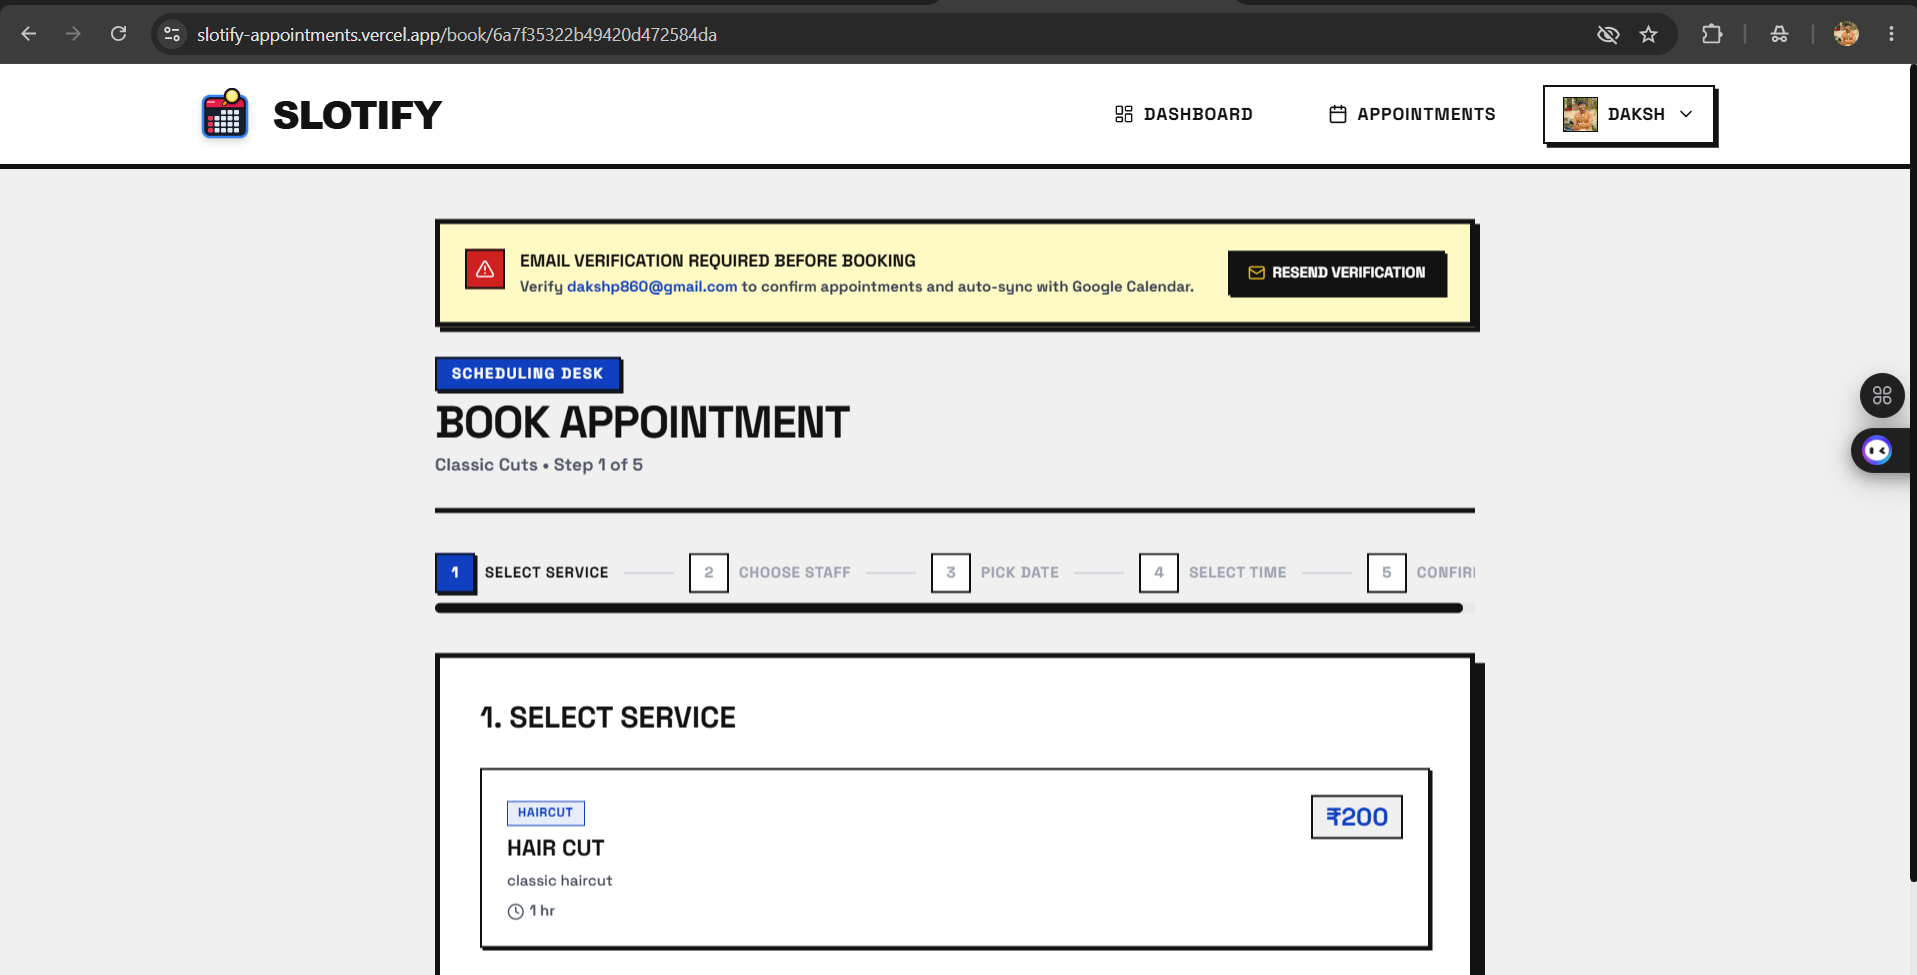
\includegraphics[width=0.85\textwidth]{images/appoinment lifecycle.png}
\caption{Appointment lifecycle flow from booking to service completion}
\end{figure}
